\section{论文的主要内容和技术路线}

\subsection{主要研究内容}
本课题旨在构建一个端到端的视觉语言导航系统（VLN-R1），重点围绕以下核心内容展开：
\begin{enumerate}
    \item \textbf{多模态感知与4-View特征适配}：针对真实机器人硬件（如搭载Seeker四目相机的移动底盘）与仿真环境（Matterport3D 12-View全景）的观测差异，研究从ResNet/CLIP\cite{radford2021learning}向\textbf{DINOv2}\cite{dinov2}视觉编码器的迁移技术。利用DINOv2的几何特征提取能力，结合坐标系对齐与特征蒸馏，实现从12-View到4-View的高效适配。同时，引入单目深度估计技术，进一步增强机器人对三维环境的感知精度。
    \item \textbf{面向连续控制的VLN-Ego数据集构建}：借鉴Aux-Think\cite{aux_think}、Nav-R1\cite{nav_r1}和OctoNav\cite{octonav}的CoT数据构建方法论，基于Habitat模拟器\cite{savva2019habitat}复用RxR\cite{ku2020rxr}数据集的离散轨迹。参考Aux-Think的R2R-CoT-320k数据集构建流程，利用\textbf{Qwen3-VL-32B-Thinking}模型生成包含空间推理过程的"思维链（CoT）"描述。采用OctoNav提出的TBA（Think-Before-Action）格式（\texttt{<Think>...</Think>}\texttt{<Action>...</Action>}），构建包含"图像序列-语言-思维链-动作"四元组的VLN-Ego数据集。根据Aux-Think的发现，CoT将作为\textbf{训练时的辅助监督信号}，而非测试时的显式推理，从而避免测试时推理崩溃（TRC）问题。
    \item \textbf{基于GRPO的强化学习微调}：针对长序列动作生成（Long-Horizon Action Generation）中的训练不稳定性，摒弃传统的PPO算法，设计并实现\textbf{组相对策略优化（Group Relative Policy Optimization, GRPO）}\cite{deepseek_r1}算法。GRPO通过组内样本的相对优势估计，显著降低了方差，提升了训练稳定性。引入长短期记忆采样（Long-Short Memory Sampling）以突破显存瓶颈，并设计时间衰减奖励（Time-Decayed Reward），在保证指令遵循准确性的同时提升导航效率。该方法已在DeepSeek-R1\cite{deepseek_r1}等大规模推理模型中验证了其在长序列生成任务中的有效性。
\end{enumerate}

\subsection{技术路线}
本研究的技术路线主要分为三个阶段：
\begin{enumerate}
    \item \textbf{阶段一：数据引擎与环境搭建}
    \begin{itemize}
        \item 搭建Habitat-Sim仿真环境，加载Matterport3D场景数据。
        \item 考虑到我们微调大模型和habit的环境冲突，我们开发自动化脚本（ETPNav-DataGen），离线预处理数据集。
        \item 部署VLM（Qwen3-VL-32B-Thinking）对关键帧进行各种视角的描述生成，构建CoT推理链。
    \end{itemize}
    \item \textbf{阶段二：模型构建与感知迁移}
    \begin{itemize}
        \item \textbf{视觉前端升级}：基于Qwen3-VL-2B-Thinking模型，将默认的clip编码器替换为DinoV2。
        \item \textbf{视场角适配}：计算仿真器相机与实车Seeker相机的内参/外参矩阵，设计坐标系对齐算法。
        \item \textbf{监督微调（SFT）}：在VLN-Ego数据集上进行LoRA微调，训练模型输出规范化的JSON动作指令（包含$v, \omega$）。
    \end{itemize}
    \item \textbf{阶段三：多阶段强化微调（参考Nav-R1、OctoNav）}
    \begin{itemize}
        \item \textbf{Action-SFT阶段}：在VLN-Ego数据集上进行监督微调，使模型学会根据指令和观测输出动作。
        \item \textbf{TBA-SFT阶段}：利用CoT数据进行Think-Before-Action微调，训练模型在输出动作前生成推理过程，作为冷启动阶段。
        \item \textbf{Nav-GRPO阶段}：参考Nav-R1\cite{nav_r1}和OctoNav\cite{octonav}的设计，基于序列似然比率实现GRPO Loss。设计三维奖励函数：（1）\textbf{格式奖励}：确保输出符合规定格式；（2）\textbf{理解奖励}：评估语义正确性和视觉接地；（3）\textbf{导航奖励}：优化路径保真度和终点准确性（SPL + TDR）。
        \item \textbf{虚实迁移}：在仿真中引入图像噪声（Motion Blur）和深度噪声，模拟真实Seeker相机的成像特性，验证模型的鲁棒性。
    \end{itemize}
\end{enumerate}

\subsection{核心方法详解}
\subsubsection{系统架构设计}
本课题提出的VLN-R1系统采用基于拓扑图的导航架构（见图\ref{fig:framework}），主要包括以下模块：
\begin{itemize}
    \item \textbf{视觉编码器}：采用ViT-B/32 (CLIP),以后的实验考虑dino,编码RGB图像，ResNet-50编码深度图像。CLIP编码器提供语义特征，深度编码器（预训练于PointGoal导航任务）提供空间几何特征。
    \item \textbf{拓扑地图模块}：在线构建环境的拓扑图表示$G_t = \langle N_t, E_t \rangle$，通过路点预测器生成候选导航节点，支持全局规划与回溯纠错。
    \item \textbf{跨模态规划模块}：基于Qwen3-VL-2B-Thinking的语言理解能力，结合图感知自注意力（GASA）机制，在拓扑图上进行目标预测和路径规划。
    \item \textbf{低级控制器}：将高层规划转换为底层动作，采用Tryout启发式机制处理障碍物避让。
\end{itemize}

\begin{figure}[htbp]
    \centering
    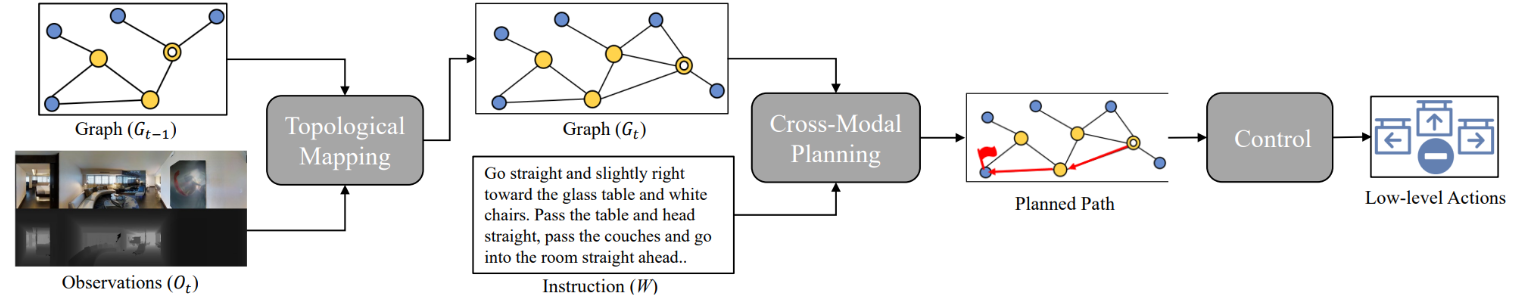
\includegraphics[width=0.9\textwidth]{figure/framework.png}
    \caption{VLN-R1系统架构设计图}
    \label{fig:framework}
\end{figure}

整体数据流为：$\text{RGBD全景图像} + \text{语言指令} \xrightarrow{\text{拓扑建图}} \text{图表示} \xrightarrow{\text{跨模态规划}} \text{导航目标} \xrightarrow{\text{控制}} \text{动作序列}$。

\subsubsection{GRPO强化学习算法}
组相对策略优化（GRPO）是一种针对长序列生成任务的改进RL算法。其核心思想是在每个训练batch内，通过组内样本的相对排序来估计优势函数，从而降低方差。

\textbf{数学形式}：给定策略$\pi_\theta$，对于每个轨迹$\tau_i = (s_0, a_0, \ldots, a_T)$，传统PPO需要估计价值函数$V(s)$并计算优势$A(s,a) = Q(s,a) - V(s)$。GRPO则通过组内归一化简化这一过程：
\[
A_i^{\text{GRPO}} = \frac{R_i - \bar{R}}{\sigma_R + \epsilon}
\]
其中$R_i$是第$i$条轨迹的累积奖励，$\bar{R}$和$\sigma_R$分别是batch内的均值和标准差。这种相对优势估计避免了显式的价值网络训练，显著提升了稳定性。

\textbf{序列级目标函数}：
\[
\mathcal{L}_{\text{GRPO}} = \mathbb{E}_{\tau \sim \pi_\theta} \left[ \min\left( r(\theta) A^{\text{GRPO}}, \text{clip}(r(\theta), 1-\epsilon, 1+\epsilon) A^{\text{GRPO}} \right) \right]
\]
其中$r(\theta) = \frac{\pi_\theta(\tau)}{\pi_{\theta_{\text{old}}}(\tau)}$是轨迹级的重要性采样比率。

\subsubsection{4-View特征适配与深度估计}
针对仿真环境的12-View全景图像与真实Seeker相机的4-View观测差异，设计了以下适配方案：
\begin{itemize}
    \item \textbf{坐标系对齐}：通过相机内参标定，建立仿真器相机坐标系与Seeker相机坐标系的映射关系。利用旋转矩阵$\mathbf{R} \in SO(3)$和平移向量$\mathbf{t} \in \mathbb{R}^3$，将12-View中的4个等效视角提取出来用于训练。
    \item \textbf{深度信息增强}：集成FoundationStereo单目深度估计模型，为每帧图像生成深度图。深度信息通过额外的depth token注入视觉编码器，帮助模型理解三维空间结构。
    \item \textbf{数据增强}：在训练阶段引入运动模糊、高斯噪声、深度量化误差等仿真到真实（Sim-to-Real）的domain gap模拟，提升模型鲁棒性。
\end{itemize}

\subsubsection{拓扑地图构建模块}
借鉴ETPNav\cite{etpnav}与Bridging the Gap\cite{bridging_gap}的设计思想，本研究引入在线拓扑地图构建机制（见图\ref{fig:topo_module}），将环境抽象为图表示$G_t = \langle N_t, E_t \rangle$：

\begin{figure}[htbp]
    \centering
    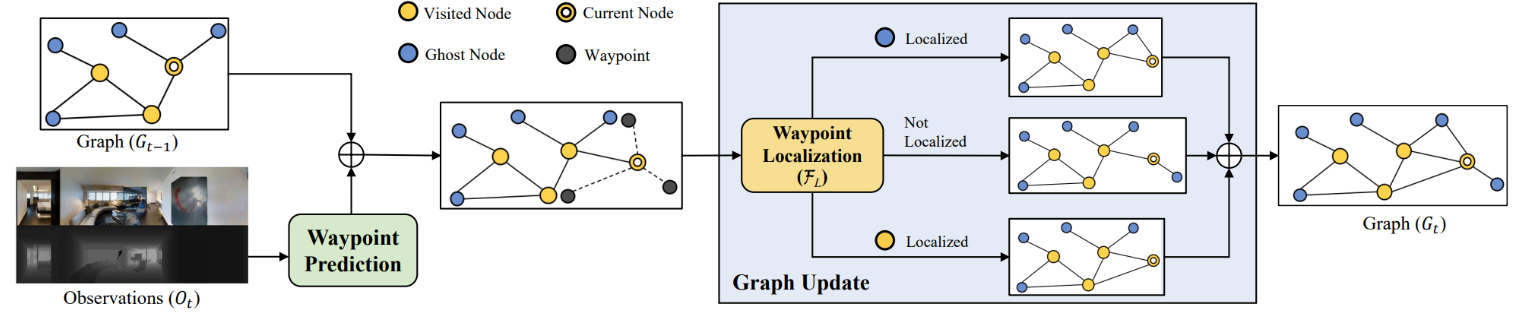
\includegraphics[width=0.9\textwidth]{figure/topo_module.png}
    \caption{拓扑地图构建与更新模块详解}
    \label{fig:topo_module}
\end{figure}

\textbf{路点预测}：采用基于Transformer的路点预测器，仅使用深度特征$V_t^d$和方向特征$V_t^{ori}$作为输入。实验表明，纯深度输入比RGBD输入在unseen环境中泛化更好。预测器输出热力图表示附近$K$个可能的路点位置$\triangle P_w = \{\triangle p_i^w\}_{i=1}^K$。

\textbf{图更新机制}：使用路点定位函数$F_L$将预测的路点与现有节点关联。若路点与现有节点的欧氏距离小于阈值$\gamma$（本研究取$\gamma=0.5$m），则累积更新该节点的表示；否则创建新的ghost节点。节点分为三类：
\begin{itemize}
    \item \textbf{已访问节点（Visited Nodes）}：智能体已经到达过的位置
    \item \textbf{当前节点（Current Node）}：智能体当前所在位置
    \item \textbf{幽灵节点（Ghost Nodes）}：已观测但未探索的位置，作为候选目标
\end{itemize}

\subsubsection{跨模态规划模块}
跨模态规划模块负责在拓扑地图上进行目标预测和路径规划：

\textbf{图感知自注意力（GASA）}：在节点编码时引入图拓扑结构，使注意力计算考虑空间关系：
\[
\text{GASA}(X) = \text{softmax}\left(\frac{XW_q(XW_k)^\top}{\sqrt{d}} + EW_e\right)XW_v
\]
其中$E$是由图边构建的节点间最短距离矩阵，$W_q, W_k, W_e, W_v$是可学习参数。

\textbf{长程目标预测}：模型预测每个ghost节点作为导航目标的得分$s_i = \text{FFN}(\tilde{n}_i)$。选择得分最高的节点作为长程目标后，通过Dijkstra算法在拓扑图上规划最短路径，生成子目标序列$P_t = \{p_m\}_{m=1}^M$。

\subsection{实验设计与评估方法}
\subsubsection{数据集与评估指标}
本研究在R2R-CE和RxR-CE两个标准基准上进行实验：
\begin{itemize}
    \item \textbf{R2R-CE}：5,611条最短路径轨迹，平均路径长度9.89m，平均指令32词，允许sliding
    \item \textbf{RxR-CE}：多语言（英语/印地语/泰卢固语）指令，平均路径长度15.23m，平均指令120词，禁止sliding
\end{itemize}

采用以下标准评估指标：
\begin{itemize}
    \item \textbf{SR（Success Rate）}：终点距目标3m内的成功率
    \item \textbf{SPL（Success weighted by Path Length）}：考虑路径效率的成功率
    \item \textbf{NE（Navigation Error）}：终点到目标的平均测地距离
    \item \textbf{nDTW / SDTW}：路径保真度指标，衡量与参考轨迹的一致性
\end{itemize}

\subsubsection{基线方法与消融实验}
将与以下方法进行对比：CWP-RecBERT\cite{bridging_gap}、ETPNav\cite{etpnav}、BEVBert、HNR等当前SOTA方法。同时设计以下消融实验验证各模块的贡献：
\begin{enumerate}
    \item 视觉编码器消融：DINOv2 vs CLIP vs ResNet
    \item 训练策略消融：SFT only vs SFT+GRPO
    \item 路点预测器输入：Depth-only vs RGBD
    \item 规划空间：全局规划 vs 局部规划
\end{enumerate}

\subsection{可行性分析}
\begin{enumerate}
    \item \textbf{技术可行性}：本项目基于目前最先进的开源多模态大模型（Qwen3-VL-2B-Thinking）构建。实验室已积累了基于Seeker相机的硬件调试经验，验证了4-View图像采集与处理通路。CLIP和DINOv2\cite{dinov2}等预训练模型的引入大大降低了从零训练感知模块的难度。
    \item \textbf{方法可行性}：GRPO算法\cite{deepseek_r1}已在DeepSeek-R1等大规模推理模型中证明了其训练稳定性，理论上完全适用于长序列的导航决策任务。长短期记忆采样策略符合人类的认知导航机理。
    \item \textbf{数据与算力}：实验室拥有完整的RxR\cite{ku2020rxr}数据集授权，以及A6000高性能计算服务器，足以支持2B参数模型的全量SFT与RL训练。
\end{enumerate}

\subsection{创新点}
\begin{enumerate}
    \item \textbf{基于DINOv2的4-View特征适配技术}：首次在VLN任务中系统地研究了从仿真全景到真实有限视角的特征迁移问题，提出了结合坐标系对齐与DINOv2几何特征的解决方案。
    \item \textbf{端到端连续控制与GRPO微调}：创新性地将组相对策略优化（GRPO）引入具身导航领域，解决了传统RL算法在长序列动作生成中的模式崩塌（Mode Collapse）问题。相比PPO，GRPO通过组内相对比较机制，大幅降低了奖励估计的方差，使得长时程导航任务的训练更加稳定高效。
    \item \textbf{可解释的CoT导航决策}：通过在训练数据中显式引入思维链（CoT），实现了"感知-推理-行动"的一体化，增强了导航过程的可解释性。
\end{enumerate}
